\chapter{Auswertungsmöglichkeiten}\label{ausblick}
\thispagestyle{fancy}

Da \textit{JCorrelat} wohl formatierte Daten in \textit{elasticsearch} ablegt, ist es 
möglich mit einer Vielzahl an weiteren Werkzeugen diese Daten zu analysieren und zu 
visualisieren. Aus diesem Grund wurde auf der Basis von \cite{kleindienst} ein 
ELK-Stack aufgebaut um weitere beispielhafte Visualisierungen vorzustellen. Der 
Aufbau des verwendeten ELK-Stacks ist Schematisch in Abbildung \ref{app:demo-elk} (Anhang)
dargestellt. Für die Visualisierung zeigt sich \textit{Kibana} verantwortlich.\\
Abbildung \ref{pic:elk-01} zeigt eine durch \textit{Kibana} erstellte Visualisierung. 
\textit{Kibana} greift dazu auf Daten zurück die durch \textit{Logstash} strukturiert in 
\textit{elasticsearch} abgelegt wurden.
Ähnlich wie im Beispielszenario (Abschnitt \ref{szenario}) sind auch hier fehlgeschlagene 
SSH-Logins anschaulich gemacht. Die IP-Quelladressen wurden dabei mithilfe von 
\textit{Geotargeting} einer möglichen Region zugewiesen, ebenso die Anzahl der 
erfolglosen Loginversuche aus dieser Region über einen vorher definierten Zeitraum. Der 
Kreisdurchmesser hat keinerlei Bedeutung, lediglich der Farbverlauf gibt in fünf 
dynamisch errechneten Abstufungen die Anzahl der erfolglosen Versuche an, wie man am 
Beispiel Kiev deutlich sieht. Um auch alle Erfolgreichen Logins anzuzeigen ist eine 
weitere Karte notwendig (Abbildung \ref{pic:elk-02}).\\
Diese Form der Illustration würde sich auch für \textit{JCorrelat} anbieten, dann 
könnten die Ereignisse (Bruet-Force-Attacke und erfolgreicher Login während einer Attacke)
auf einer Karte darstellt werden.

\begin{figure}[htbp]
    \caption{Visualisierung mit Kibana (fehlgeschlagene Logins)}
    \label{pic:elk-01}\vspace{0.2cm}
    \centering
    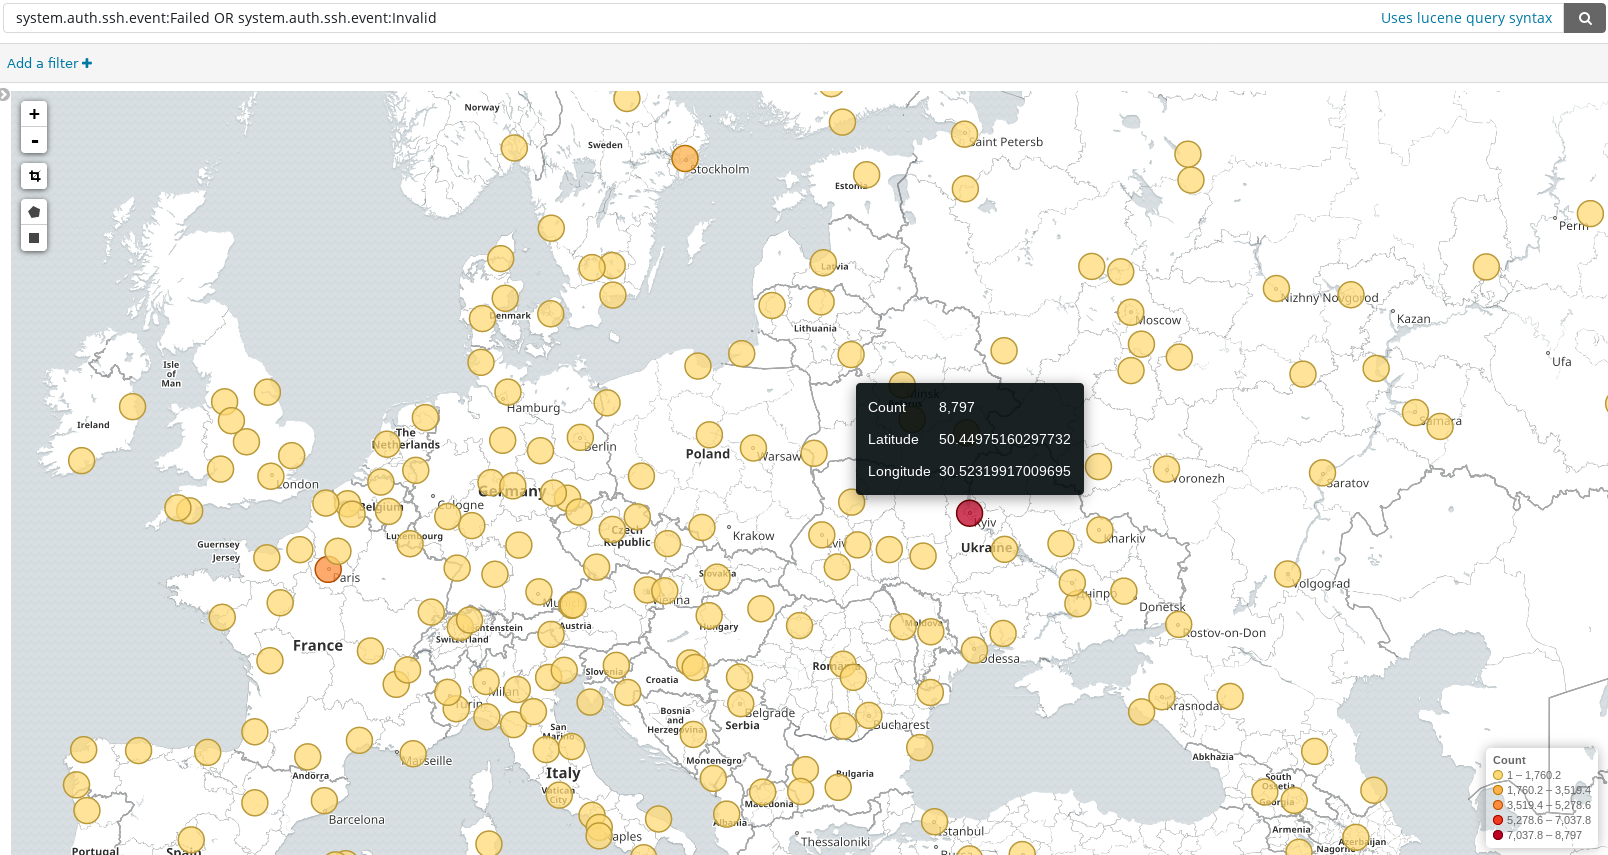
\includegraphics[scale=0.28]{img/elk-01}  
\end{figure}

\begin{figure}[htbp]
    \caption{Visualisierung mit Kibana (erfolgreiche Logins)}
    \label{pic:elk-02}\vspace{0.2cm}
    \centering
    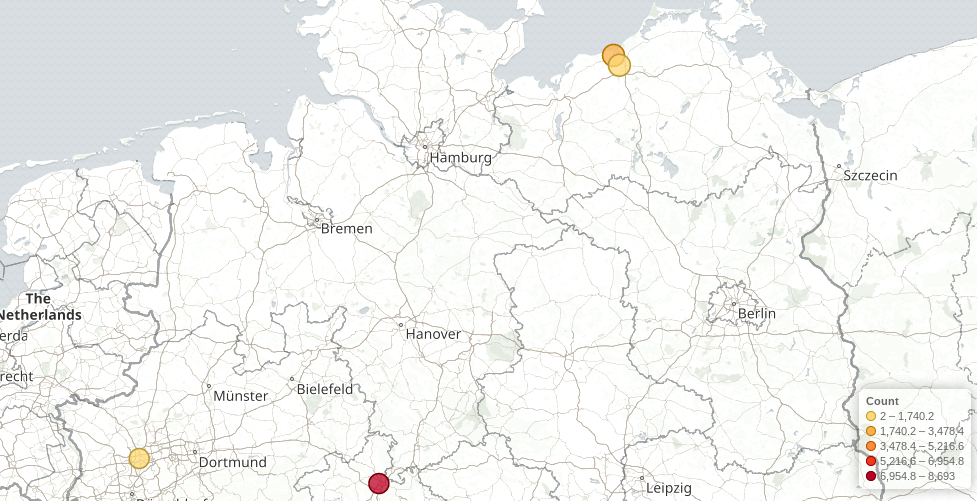
\includegraphics[scale=0.33]{img/elk-02}  
\end{figure}